\documentclass[a4paper,12pt]{article} 
\usepackage[T2A]{fontenc}			
\usepackage[utf8]{inputenc}			
\usepackage[english,russian]{babel}	
\usepackage{amsmath,amsfonts,amssymb,amsthm,mathrsfs,mathtools} 
\usepackage{cancel}
\usepackage{hhline}
\usepackage{multirow}
\usepackage[colorlinks, linkcolor = purple, citecolor = purple]{hyperref}
\usepackage{upgreek}\usepackage[left=2cm,right=2cm,top=2cm,bottom=3cm,bindingoffset=0cm]{geometry}
\usepackage{tikz}
\usepackage{graphicx}
\graphicspath{ {./pictures/} }
\usepackage{subfig}
\usepackage{titletoc}
\usepackage{tikz}
\usepackage{pgfplots}
\usepackage{xcolor}
\usepackage{wrapfig}
\usepackage{todonotes}

\newcommand\myworries[1]{\colorbox{red!30}{TODO #1}}
\newcommand\attention[1]{\colorbox{cyan!30}{#1}}

\title{Sem8Synopsis}
\author{Александр Мишин, Б01-008а}
\date{}
\begin{document}

\maketitle

\attention{Новое дз было закинуто в беседу, сделать!!}
\section{Интерполяция по кратным узлам}
По набору точек мы можем провести полином той или иной степени. В полиноме Ньютона не совсем готовая формула, в полиноме Лагранжа - всё сразу готово. Подробнее - прошлый семинар. С точки зрения программирования, полином Лагранжа - не очень. А вот полином Ньютона - кайф чистый. Также мы говорили, что через две точки можно провести не только прямую (с точки зрения вычматов). Можно провести всё.\\

Кратный узел - узел, в котором задано кол-во значений производных при том, что задано значение функции. Задано только f - кратность ?. Задано ещё f' - кратность ?+1.\\


\begin{table}[h!]
\centering
\begin{tabular}{|l|l|r|r|}
\hline
x     & \multicolumn{1}{r|}{1}  & 2 & 3                     \\ \hline
f(x)  & \multicolumn{1}{r|}{-1} & 0 & 1                     \\ \hline
f'(x) &                         & 3 & 2                     \\ \hline
f"(x) &                         & 2 & \multicolumn{1}{l|}{} \\ \hline
\end{tabular}
\end{table}

Решаем методом Ньютона, значит строим табличку. Точку 2 повторяю 3 раза, точку 3 - 2 раза. Дальше точно так же нахожу $b_0$, $b_1$, $b_2$. Разделённая разность обозначалась $f(x_i, x_{i-1})$. Когда мы ищем $f(x_i, x_i)$, то используем 
\[f(x_i, ...) = \frac{f^{(k)}}{k!}\]

\begin{table}[h!]
\centering
\begin{tabular}{|r|r|r|r|l|l|l|}
\hline
\multicolumn{1}{|c|}{x} & \multicolumn{1}{c|}{b_0} & \multicolumn{1}{c|}{b_1} & \multicolumn{1}{c|}{b_2} & \multicolumn{1}{c|}{b_3} & \multicolumn{1}{c|}{b_4} & \multicolumn{1}{c|}{b_5} \\ \hline
\attention{-1}                      & \attention{-1}                        & \multicolumn{1}{l|}{}     & \multicolumn{1}{l|}{}     &                           &                           &                           \\ \hline
2                       & 0                         & \attention{1}                         & \multicolumn{1}{l|}{}     &                           &                           &                           \\ \hline
2                       & 0                         & 3                         & \attention{2}                         &                           &                           &                           \\ \hline
2                       & 0                         & 3                         & f"(2) / 2! = 1            & \multicolumn{1}{r|}{\attention{-1}}   &                           &                           \\ \hline
3                       & 1                         & 1                         & -2                        & \multicolumn{1}{r|}{-3}   & \multicolumn{1}{r|}{\attention{-1}}   &                           \\ \hline
3                       & 1                         & 2                         & 1                         & \multicolumn{1}{r|}{3}    & \multicolumn{1}{r|}{6}    & \multicolumn{1}{r|}{\attention{3.5}}  \\ \hline
\end{tabular}
\end{table}

Следовательно, строим полином пятой степени. Построим полином Эрмита Н.

\[H_5(x) = -f + 1\cdot(x-1) + 2\cdot(x-1)(x-2) +(-1)\cdot(x-1)(x-2)^2 + (-1)\cdot(x-1)(x-2)^3 + 3.5\cdot(x-1)(x-2)^3(x-3)\]

Одним из способов уменьшения ошибки при решении является использование Чебышёвской интерполяции, делая сетку неравномерной.
\section{Сплайн-интерполяция}
В чём основная идея? На каждом отрезочке есть две идеи - локальная Сплайн интерполяции и глобальный.

    \begin{figure}[h!]
        \centering
        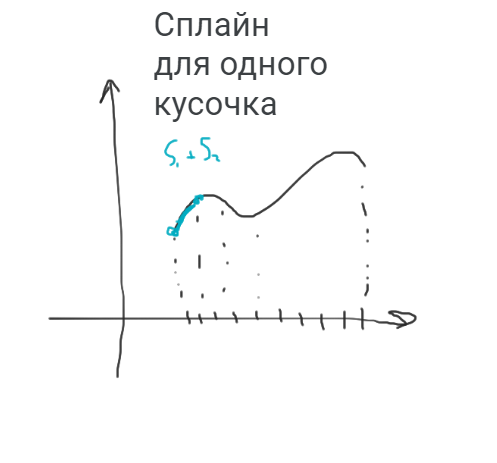
\includegraphics[width=12cm]{8semPic1.png}
    \end{figure}

Есть также глобальный сплайн, где задание интерполяции большой кривой S.

\subsection{Пример}

\begin{table}[h!]
\centering
\begin{tabular}{|l|r|r|r|}
\hline
x & 0 & 1 & 2 \\ \hline
f & 1 & 0 & 2 \\ \hline
\end{tabular}
\end{table}

$$f'(0) = 0$$
$$f"(0) = 0$$

Требуется локальный кубический сплайн. 

Решение.\\
\[S_1 = a_3x^3 + a_2x^2 + a_1x + a_0\]
\[S_2 = b_3x^3 + b_2x^2 + b_1x + b_0\]

Ищем уравнения.\newpage

\[S_1(0) = 1\]
\[S_1(1) = 0\]
\[S_2(1) = 0\]
\[S_2(2) = 2\]
\[S'_1(0) = 0\]
\[S"_1(0) = 0\]
\[S'_1(1) = S'_2(1)\]
\[S"_1(1) = S"_2(1)\]

Отсюда находим все $a_i, b_i$.
\[S_1 = -x^3 + 1\]
\[S_2 = 8x^3 - 27x^2 + 27x - 8\]
В сумме это и есть наш сплайн S(x) = $S_1(x) + S_2(x)$. 

\subsection{Теорема о построении, существовании и единственности естественного сплайна.}
Пусть на неком [a, b] задана непрерывная f(x) и система узлов {x_k}, $k =\overline{0, m}; x_0 = a; x_n = b; h_i = x_i - x_{i-1}$

Пусть\\
1) $S_k(x) = f(x_k)$ - условие интерполяции\\
2)$S_k(x) \in C^2[a;b]$\\
3) Для каждого отрезка [$x_k, x_{k+1}] : S(x) = \sum_0^3 a_j x_j$\\
4) Краевые условия для S(x) представляются одним из следующих видов:\\
\begin{itemize}
    \item S'(a) = f'(a); S'(b) = f'(b)
    \item S"(a) = f"(a); S"(b) = f"(b)
    \item S(a) = S(b)
    \item S'(a) = S'(b)
\end{itemize}
Тогда существует и единственный сплайн 3-го подрядко с дефектом 1.\\

Дефект = степень полиномов - кол-во произв.\\
Естественный сплайн - такой, что S"(a) = 0; S"(b) = 0\\

\[S_k = a_k + b_k(x-x_k) + \frac{c_k}{2}(x-x_k)^2 + \frac{d_k}{6}(x-x_k)^3\]

\end{document}
